\documentclass[12pt,a4paper]{article}

\usepackage[T1]{fontenc}
\usepackage[polish]{babel}
\usepackage[utf8]{inputenc}
\usepackage{lmodern}
\selectlanguage{polish}
\usepackage{graphicx}
\usepackage{biblatex}
\usepackage{csquotes}
\usepackage{listings}
\usepackage{color}
\definecolor{bluekeywords}{rgb}{0.13,0.13,1}
\definecolor{greencomments}{rgb}{0,0.5,0}
\definecolor{redstrings}{rgb}{0.9,0,0}
\graphicspath{ {./media/} }
\lstset{
breaklines,
language=[Sharp]C,
showspaces=false,
showtabs=false,
showstringspaces=false,
breakatwhitespace=true,
escapeinside={(*@}{@*)},
commentstyle=\color{greencomments},
keywordstyle=\color{bluekeywords}\bfseries,
stringstyle=\color{redstrings},
basicstyle=\ttfamily
breaklines
}

\begin{document}


\nocite{*}

\pagenumbering{gobble}
\clearpage
\hspace{3cm}
\begin{center}POLITECHNIKA ŚLĄSKA W GLIWICACH\end{center}
\begin{center}Wydział Matematyki Stosowanej\end{center}
\begin{center}Kierunek: Informatyka\end{center}
\begin{center}Magisterskie, stacjonarne, sem. II\end{center}
\hspace{3cm}
\begin{center}\large\textbf{DOKUMENTACJA PROJEKTU Z PRZEDMIOTU\\MODELOWANIE I ANALIZA SYSTEMÓW INFORMATYCZNYCH}\end{center}
\hspace{10cm}
\begin{center}TEMAT ZADANIA: SYSTEMY AGENTOWE\end{center}
\hspace{5cm}
\begin{flushright}Członkowie zespołu:
\par
\textit{Bartosz Ociepka}
\par
\textit{Beniamin Stecuła}
\end{flushright}
\vfill
\begin{center}Internet, 2020/2021\end{center}

\newpage
\section{Podział pracy}

\begin{center}Bartosz Ociepka - backend\\Beniamin Stecuła - frontend, dokumentacja\end{center}



\section{Udokumentowanie prac}
	Dokumentowanie pracy odbyło się na kilka sposobów:
\begin{itemize}
	\item utworzenie niniejszej dokumentacji,
	\item zarządzanie podziałem i wykonaniem zadań w serwisie Trello,
	\item przechowywanie kopii poprzednich wersji programu.
\end{itemize}

W ramach repozytorium każdy z nas wrzucał commity do swoim zadań \\
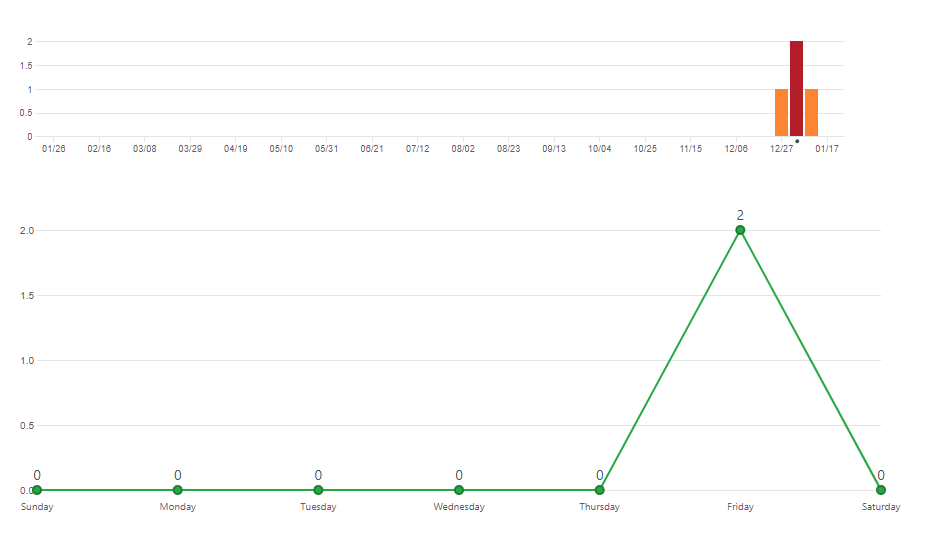
\includegraphics[width=0.9\linewidth]{media/githubProof}\\
Całe repozytorium jest dostępne pod adresem \\https://github.com/BartoszOciepka/DiabetesNeuralNetwork




\section{Założenia projektu}




\section{Cel projektu}




\section{Instrukcja wdrażania projektu}




\section{Instrukcja obsługi projektu}
Aby uruchomić nasz projekt wystarczy kliknąć przycisk Play w Unity. Wcześniej jednak należy upewnić się, że w każdym z graczy jest odpowiedni model sieci neuronowej oraz jest wybrany odpowiedni tryb gry (\textit{Training} - dla odradzania się, \textit{Inferencing} dla jednego życia każdego z graczy) oraz tryb sterowania (\textit{Default} - sterowanie przez AI, \textit{Heurisitic} - sterowanie 'strzałkami').




\section{System agentowy}
W naszym projekcie mamy 2 rodzaje agentów.\\
Pierwszym rodzajem jest gracz. Każdy gracz pozostawia za sobą 'ścianę'. Wjechanie w 'ścianę' powoduje koniec gry (tak samo jak wjechanie w ściany określające koniec areny). W ramach biblioteki ML Agents nasi gracze są wyposażeni w sztuczną inteligencję opartą o uczenie przez wzmacnianie. Agenci są w nim punktowani za każdy ruch który nie doprowadza do ich śmierci oraz unieszkodliwienie przeciwnika własną ścianą, za co dostają bardzo duży bonus. Sieć neuronowa ma 3 warstwy, a w każdej z nich po 128 neuronów (pełna konfiguracja znajduje się w pliku Assets/AI/Tron.yaml). Agenci mają sensory co 45 stopni w każdym kierunku i na tej podstawie określają co się obok nich znajduje (domyślnie widzą na 20 jednostek w przód). Sieć sprawdza też położenie przeciwnika (jeśli jest na tyle blisko żeby był widziany przez agenta). Każdy z tych agentów dokonuje akcji co 20 klatek animacji. Ten typ agenta możemy również uruchomić w trybie pozwalającym na samodzielne kierowanie.\\
Kolejnym typem agenta jest wieża. Wieża nie bierze udziału w rozgrywce lecz ma ogląd na całą arenę i może pomagać lub przeszkadzać graczom. Co pewien losowy czas (od 1 do 10 sekund) wieża wysyła graczom koordynaty jego przeciwnika. Na początku jednak wieża losowo wybiera dla każdego gracza czy mu pomaga (podaje poprawne koordynaty) czy przeszkadza (podając losowe). Gracze domyślnie wierzą wieży lecz jeśli zauważą odstępstwo między lokalizacją przeciwnika widzianą przez nich a podawaną przez wieżę to przestają i do końca gry nie reagują na jej 'pomoc'.




\section{Wady i zalety systemów agentowych}
Na podstawie implementowanego projektu możemy wyciągnąć wnioski co do systemów agentowych. Przede wszystkim uczenie przez wzmacnianie (ang. Reinforcement learning) niezbyt nadaje się do tego typu projektu. Mimo długiego uczenia wyniki nie są zadowalające. Kolejną wadą jaką dostrzegliśmy to skomplikowanie całego systemu. Sama sztuczna inteligencja to dopiero początek ponieważ oprócz tego w systemie trzeba zamodelować powiązania między agentami i ich interakcje. W naszym przypadku powodowało to, że cały system jest duży i po części jest 'black boxem' więc trudno było dostosowywać wartości w systemie aby funkcjonował on lepiej. Mimo skomplikowania dostrzegamy dużą zaletę systemów eksperckich jaką jest możliwość dostosowania do zadania. W naszym przypadku jest to gra typu Tron, ale w sieci bez problemu można znaleźć modele agentowe w innych grach lub innych systemach. 




\section{Wygląd systemu}
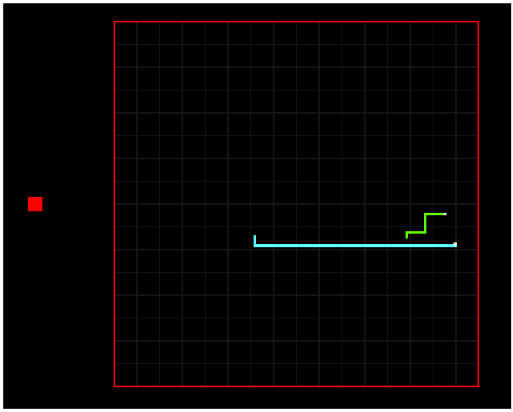
\includegraphics[scale=0.8]{media/Wyglad1}




\section{Fragmenty kodu}
TronAgent.cs
\begin{lstlisting}
using Unity.MLAgents;
using Unity.MLAgents.Sensors;
using UnityEngine;
using System;

namespace Tron
{
	[System.Serializable]
	public struct Sensor
	{
		public Transform Transform;
		public float HitThreshold;
	}

	public struct Position
	{
		public float x;
		public float y;
	}

	public enum AgentMode
	{
		Training,
		Inferencing
	}

	public enum Direction
	{
		Up = 0,
		Down = 1,
		Right = 2,
		Left = 3
	}

	public class TronAgent : Agent
	{
		public int actionCount = 0;
		public GameObject enemy;
		public Position enemyPosition;
		public float canDetectEnemyFrom;
		public bool trustTower = true;
		public bool isMyenemyLocationValid = true;
		
		#region Steering
		[Header("Steering")]
		public KeyCode upKey;
		public KeyCode downKey;
		public KeyCode rightKey;
		public KeyCode leftKey;
		#endregion
		
		#region Attributes
		[Header("Agent atributes")]
		public float speed = 16;
		public bool isAgentAlive = true;
		public Direction direction;
		public Direction lastDirection;
		public GameObject wallPrefab;
		Collider2D wall;
		Vector2 lastWallEnd;
		public string tag;
		#endregion

		#region Training Modes
		[Tooltip("Are we training the agent or is the agent production ready?")]
		public AgentMode Mode = AgentMode.Training;
		#endregion

		#region Senses
		[Header("Observation Params")]
		[Tooltip("Sensors contain ray information to sense out the world, you can have as many sensors as you need.")]
		public Sensor[] Sensors;
		#endregion

		#region Rewards
		[Header("Rewards")]
		[Tooltip("What penatly is given when the agent crashes?")]
		public float HitPenalty;
		public float CloseCallPenalty;
		public float stayingAliveReward;
		public float rewardForKill;
		#endregion


		public override void OnActionReceived(float[] vectorAction)
		{
			base.OnActionReceived(vectorAction);
			print(name + " received action: go " + ((Direction)
			((int)vectorAction[0])).ToString());
			direction = (Direction)(int)vectorAction[0];
			actionCount++;
		}

		public void moveAgent(Direction dir)
		{
			switch (dir)
			{
				case Direction.Up:
					GetComponent<Rigidbody2D>
					().velocity = Vector2.up * speed;
					break;
				case Direction.Down: //DOWN
					GetComponent<Rigidbody2D>
					().velocity = -Vector2.up * speed;
					break;
				case Direction.Right: //RIGHT
					GetComponent<Rigidbody2D>
					().velocity = Vector2.right * speed;
					break;
				case Direction.Left: //LEFT
					GetComponent<Rigidbody2D>
					().velocity = -Vector2.right * speed;
					break;
			}

			direction = dir;
			spawnWall();
		}

		public override void Heuristic(float[] actionsOut)
		{
			actionsOut[0] = Input.GetKey(upKey) ? 0.0f : actionsOut[0];
			actionsOut[0] = Input.GetKey(downKey) ? 1.0f : actionsOut[0];
			actionsOut[0] = Input.GetKey(rightKey) ? 2.0f : actionsOut[0];
			actionsOut[0] = Input.GetKey(leftKey) ? 3.0f : actionsOut[0];
			direction = (Direction)((int)actionsOut[0]);
		}

		void changeWallDueToPlyerMove(Collider2D co, Vector2 a, Vector2 b)
		{
			if (co == null) return;
			co.transform.position = a + (b - a) * 0.5f;

			float dist = Vector2.Distance(a, b);
			if (a.x != b.x)
			{
				co.transform.localScale = new Vector2(dist + 1, 1);
			}
			else
				co.transform.localScale = new Vector2(1, dist + 1);
		}

		private void OnTriggerEnter2D(Collider2D co)
		{
			if (co != wall)
			{
				if(Mode == AgentMode.Inferencing)
				{
					KillPlayer();
				}
				else
				{
					print("Player lost: " + name);
					AddReward(HitPenalty);
					if (co.tag != tag && co.tag != "Wall") enemy.GetComponent
					<TronAgent>()
					.killedAPlayer(); //informing enemy that they were killed by him
					EndEpisode();
					ResetAgent();
				}
			}
		}

		void KillPlayer()
		{
			print("Player lost: " + name);
			Destroy(gameObject);
		}
		void spawnWall()
		{
			lastWallEnd = transform.position;
			GameObject g = Instantiate(wallPrefab, transform.position, Quaternion.identity);
			wall = g.GetComponent<Collider2D>();
		}

		public override void OnEpisodeBegin()
		{
			//GetComponent<Rigidbody2D>().velocity = Vector2.up * speed;
			//direction = 0;
			//lastDirection = 0;
			//moveAgent(direction);
			ResetAgent();
		}

		private void LateUpdate()
		{
			float bonus = (actionCount / 1000 * 5);
			changeWallDueToPlyerMove(wall, lastWallEnd, transform.position);
			 if (checkIfOppositeDirections(direction, lastDirection))
			{
				if (Mode == AgentMode.Inferencing) KillPlayer();
				else {
					print("Player lost: " + name);
					//AddReward(HitPenalty);
					EndEpisode();
					ResetAgent();
				}
			}
			else if( lastDirection != direction){
				moveAgent(direction);
				lastDirection = direction;
				//AddReward(bonus);
			}

			changeWallDueToPlyerMove(wall, lastWallEnd, transform.position);

			//AddReward(stayingAliveReward);
			AddReward(actionCount / 1000);
		}

		public bool checkIfOppositeDirections(Direction dir1, Direction dir2)
		{
			if ((dir1 == Direction.Left && dir2 == Direction.Right) ||
				(dir1 == Direction.Right && dir2 == Direction.Left) ||
				(dir1 == Direction.Up && dir2 == Direction.Down) ||
				(dir1 == Direction.Down && dir2 == Direction.Up)) return true;
			else
			{
				return false;
			}
		}

		public override void CollectObservations(VectorSensor sensor)
		{
			getEnemyPosition();
			sensor.AddObservation(enemyPosition.x);
			sensor.AddObservation(enemyPosition.y);
			sensor.AddObservation(transform.position);
			bool didHit = false;
			for (int i = 0; i < Sensors.Length; i++)
			{
				int layerMask = ~(LayerMask.GetMask("Ignore Raycast"));
				var current = Sensors[i];
				var xform = current.Transform;
				RaycastHit2D hitInfo = new RaycastHit2D();
				hitInfo = Physics2D.Raycast(current.
				Transform.position + new Vector3(0.0f, 0.0f, 0.0f), xform.up, 20, layerMask);;

				sensor.AddObservation(hitInfo);
				if (hitInfo.collider != null && hitInfo.collider != wall && hitInfo.distance < current.HitThreshold)
				{
					//AddReward
					(CloseCallPenalty);
					didHit = true;
				}
				else
				{
					
				}
			}
			if (didHit)
			{
				//ResetAgent();
			}
		}

		public void ResetAgent()
		{
			trustTower = true;
			actionCount = 0;
			float min = -60;
			float max = 60;
			float x = UnityEngine.Random.Range(min, max);
			float y = UnityEngine.Random.Range(min, max);
			transform.position = new Vector2(x, y);
			int dir = UnityEngine.Random.Range(0, 3);
			direction = (Direction)dir;
			lastDirection = (Direction)dir;
			DestroyAllObjectsWithTag(tag);
			wall = null;
			lastWallEnd = new Vector2(x, y);
			moveAgent(direction);
		}

		public void DestroyAllObjectsWithTag(string tag)
		{
			var gameObjects = GameObject.FindGameObjectsWithTag(tag);

			for (var i = 0; i < gameObjects.Length; i++)
			{
				Destroy(gameObjects[i]);
			}
		}

		public void getEnemyPosition()
		{
			Position enemyPosition = new Position();
			enemyPosition.x = enemy.transform.position.x;
			enemyPosition.y = enemy.transform.position.y;

			Position myPosition = new Position();
			myPosition.x = GetComponent<Rigidbody2D>()
			.transform.position.x;
			myPosition.y = GetComponent<Rigidbody2D>()
			.transform.position.y;

			if(calculateDistance(enemyPosition, myPosition) < canDetectEnemyFrom)
			{
				this.enemyPosition = enemyPosition;
				isMyenemyLocationValid = true;
			}
			else
			{
				isMyenemyLocationValid = false;
			}
		}

		public double calculateDistance(Position one, Position second)
		{
			return Math.Sqrt(Math.Pow(second.x - one.x, 2) + Math.Pow(second.y - one.y, 2));
		}

		public void killedAPlayer()
		{
			AddReward(rewardForKill);
		}

		public void receiveHelp(float x, float y)
		{
			Position receivedEnemyPosition = new Position();
			receivedEnemyPosition.x = x;
			receivedEnemyPosition.y = y;

			Position myPosition = new Position();
			myPosition.x = GetComponent<Rigidbody2D>()
			.transform.position.x;
			myPosition.y = GetComponent<Rigidbody2D>()
			.transform.position.y;

			if (isMyenemyLocationValid && (enemyPosition.x != receivedEnemyPosition.x || enemyPosition.y != receivedEnemyPosition.y))
			{
				trustTower = false;
			}

			if (trustTower)
			{
				enemyPosition = receivedEnemyPosition;
			}
		}
	}
}

\end{lstlisting}

TowerAgent.aspx
\begin{lstlisting}
using System.Collections;
using UnityEngine;
public class TowerAgent : MonoBehaviour
{
	public GameObject[] players = new GameObject[2];
	public bool[] helping = new bool[2];
	System.Random random = new System.Random();
	void Start()
	{
		chooseWhoToHelp();
		StartCoroutine(helpPlayers());
	}

	// Update is called once per frame
	void Update()
	{

	}

	public IEnumerator helpPlayers()
	{
		while (true)
		{
			for (int i = 0; i < players.Length; i++)
			{
				int enemyIndex;
				if (i == 0) enemyIndex = 1;
				else enemyIndex = 0;


				if (helping[i] == true) players[i].GetComponent
				<Tron.TronAgent>().receiveHelp
				(players[enemyIndex].GetComponent
				<Rigidbody2D>().transform.position.x,
					 players[enemyIndex].
					 GetComponent<Rigidbody2D>
					 ().
					 transform.position.y);
				else
					players[i].GetComponent
					<Tron.TronAgent>()
					.receiveHelp(random.
					Next(-60, 60), random.Next(-60, 60));
			}

			yield return new WaitForSeconds(random.Next(10));
		}
	}

	public void chooseWhoToHelp()
	{
		for (int i = 0; i < players.Length; i++)
		{
			if (random.Next(100) < 50)
			{
				helping[i] = true;
			}
			else
				helping[i] = false;
		}
	}
}

\end{lstlisting}

TestTronAgent.cs
\begin{lstlisting}
using System;
using Microsoft.VisualStudio.TestTools.UnitTesting;
using Tron;

namespace TronTest
{
	[TestClass]
	public class TestTronAgent
	{
		TronAgent agent = new TronAgent();
		[TestMethod]
		public void TestCorrectDistanceIsMeasured()
		{
			Position one = new Position();
			one.x = 1;
			one.y = 1;

			Position two = new Position();
			two.x = 2;
			two.y = 1;

			Assert.AreEqual(agent.
			calculateDistance(one, two), 1);
		}

		[TestMethod]
		public void TestCorrectOppositeDirectionIsShown()
		{
			Direction one = Direction.Up;
			Direction two = Direction.Down;
			Direction three = Direction.Right;

			Assert.AreEqual(agent.
			checkIfOppositeDirections(one, two), true);
			Assert.AreEqual(agent.
			checkIfOppositeDirections(one, three), false);
		}
	}
}

\end{lstlisting}

\end{document}
